\chapter{Association Analysis}

Association analysis is a field of techniques aimed at extracting interesting relationships hidden in large datasets. A common application of association analysis is for market basket transactions, which is data referring to purchases done by customers in shops. This data is typically in the form of a set of rows, one per transaction, each containing the set of items bought by a given customer during a single trip. This information can be used to study purchasing habits in order to support a variety of business-related applications, such as marketing promotions, inventory management, and customer relationship management.

\section{Terminology}

Before explaining any algorithm, we need to define some useful terms. As mentioned before, the data is organized into transactions. Let $I$ be the set of all items, and $T$ the set of all transactions. Each transaction $t_i$ contains a number of subsets of $I$, called an \textbf{itemsets}: $t_i = \{ X_1, X_2, \dots, X_n \}$, $X_j = \{ i_1, i_2, \dots, i_k \}$. An itemset containing $k$ items is also called a \textbf{$k$-itemset}. An itemset with no elements is called the null (or empty) itemset. A transaction $t_i$ contains an itemset $X$ if $X$ is a subset of $t_i$.

An important property of an itemset is its support count.

\BoxDef{Support Count}{
The support count of an itemset $X$ is calculated as:
\begin{equation*}
    \sigma(X) = \#\{ t_i | X \subseteq t_i, t_i \in T \}
\end{equation*}
}
In other words, the support count is the number of transactions that contain that itemset. Often, the property of interest is the support.

\BoxDef{Support}{
The support of an itemset $X$ is calculated as:
\begin{equation*}
    s(X) = \dfrac{\sigma(X)}{N}
\end{equation*}
}
An itemset is deemed \textbf{frequent} if its support $s(X)$ is greater than some used-defined minimum threshold, \textit{minsup}.

\BoxDef{Association Rule}{
An association rule is an implication expression between two disjoint itemsets $X$ and $Y$:
\begin{equation*}
    X \rightarrow Y
\end{equation*}
$X$ is called the antecedent, $Y$ the consequent.
}
The strength of an association rule can be measured both in terms of support, and \textbf{confidence}.

\BoxDef{Support of Rule}{
The support of an association rule $X \rightarrow Y$ is calculated as:
\begin{equation*}
    s(X \rightarrow Y) = \dfrac{\sigma(X \cup Y)}{N}
\end{equation*}
}

\BoxDef{Confidence of Rule}{
The confidence of an association rule $X \rightarrow Y$ is calculated as:
\begin{equation*}
    c(X \rightarrow Y) = \dfrac{\sigma(X \cup Y)}{\sigma(X)}
\end{equation*}
}
Support determines how often a rule is applicable to a given dataset, while confidence determines how frequently items in $Y$ appear in transactions that contain $X$.

The goal of association analysis is to extract all rules whose support and confidence are higher than \textit{minsup} and \textit{minconf}, respectively. The brute force approach, in which all possible rules are generated and classified as frequent or infrequent, is highly computationally expensive: for a given dataset of $d$ items, we can list a total of $3^d - 2^{d+1} + 1$ association rules.

Typically, association analysis is broken into two steps: \textbf{frequent itemset generation}, which finds all itemsets with an high enough support, and \textbf{rule generation}, which generates rules based on the frequent itemsets found in the previous step, keeping only the ones with high enough confidence.

\section{Frequent Itemset Generation}

In general, a dataset that contains $k$ items can generate up to $2^k - 1$ itemsets (excluding the empty set). Since $k$ is often very big, the search space of itemsets is too large to be explored exhaustively. The brute-force approach to generate all possible itemsets and calculating support for each of them has a complexity of $O(NMw)$, where $N$ is the number of transactions, $M$ is the number of candidate itemsets, and $w$ is the maximum transaction width (i.e., the number of item a transaction contains). The most common efficient solution to the problem is based on the \textbf{Apriori principle}.

\BoxDef{Apriori principle}{
If an itemset is frequent, then all of its subsets must also be frequent.
}

This principle also implies that if an itemset is infrequent, then all of its supersets will also be infrequent. Consider the example dataset represented by the table below:

\begin{table}[h]
    \centering
    \begin{tabular}{|c|c|}
    \hline
        TID & Items \\
    \hline
        1 & $A$, $B$, $C$ \\
    \hline
        2 & $B$, $D$, $E$, $F$ \\
    \hline
        3 & $C$, $D$, $F$ \\
    \hline
        4 & $B$, $E$, $F$ \\
    \hline
        5 & $A$, $B$, $E$, $F$ \\
    \hline
    \end{tabular}
\end{table}

Assuming a \textit{minsup} threshold of 0.6, the itemset $\{B,E,F\}$ is frequent. The itemsets $\{B,E\}$, $\{B,F\}$, and $\{E,F\}$ are frequent as well. Conversely, $\{A,B\}$ is not frequent, so any itemset obtained by adding items to it will also be infrequent.

The Apriori property holds because of the \textbf{anti-monotone property} of the support measure.

\BoxDef{Anti-monotone property}{
A measure $f$ possesses the anti-monotone property if for every itemset $X$ that is a proper subset of an itemset $Y$, it holds that $f(Y) \leq f(X)$.
}

\subsection{Apriori Algorithm}

The Apriori algorithm uses the Apriori principle to generate all potential frequent itemsets and prune infrequent ones. The pseudocode for the algorithm is presented below.

\begin{algorithm}
\caption{Frequent itemset generation of the Apriori algorithm.}
\begin{algorithmic}[1]
    \State $k = 1$
    \State $F_k = \{ i | i \in I \land s(\{i\}) \geq minsup \}$ \# find all frequent itemsets

    \Repeat
        \State $k = k + 1$
        \State $C_k$ = candidate-gen($F_{k-1}$) \# generate all candidate itemsets
        \State $C_k$ = candidate-prune($C_k$, $F_{k-1}$) \# prune itemsets with infrequent subsets

        \For{all $t \in T$}
            \State $C_t$ = subsets($C_k$, $t$)

            \For{all $c \in C_t$}
                \State $\sigma(c) = \sigma(c) + 1$ \# increment support count
            \EndFor
        \EndFor
        \State $F_k = \{ c | c \in C_k \land s(c) \geq minsup \}$ \# find all frequent k-itemsets
    \Until{$F_k = \emptyset$}
    \State \Return $\cup F_k$
\end{algorithmic}
\end{algorithm}

The algorithm starts by scanning the dataset and finding all frequent items, constructing the set of frequent 1-itemsets. The main loop can be broken into three different main phases: candidate generation, candidate pruning, and support counting.

\subsubsection{Candidate generation}

This phase generates new candidate $k$-itemsets by ``fusing'' together the frequent $(k-1)$-itemsets found in the previous iteration. The brute-force approach consists in combining all $d$ items to produce all possible $k$-itemsets, but it would result in a total of $\binom{d}{k}$ candidates.

An alternative method for candidate generation is the $F_{k-1} \times F_1$ method. Each frequent $(k-1)$-itemset is extended with frequent items that are not part of the $(k-1)$-itemset. This procedure is complete, since every frequent $k$-itemset is composed of a frequent $(k-1)$-itemset and a frequent 1-itemset. All frequent $k$-itemsets are contained within the candidate $k$-itemsets generated. Still, this procedure produces a large number of unnecessary candidates, and can produce duplicate candidates as well.

Another method is the $F_{k-1} \times F_{k-1}$ method, which is the one actually used by the Apriori algorithm. The set of candidate $k$-itemsets is obtained by merging together pairs of frequent $(k-1)$-itemsets. A pair is merged only if their first $k-2$ items, sorted lexicographically, perfectly match. More formally: let $A = \{ a_1, a_2, \dots, a_{k-1} \}$ and $B = \{ b_1, b_2, \dots, b_{k-1} \}$ be two frequent $(k-1)$-itemsets. $A$ and $B$ can be merged if and only if:
\begin{equation*}
    a_i = b_i \,, i \in [1,k-2] \,.
\end{equation*}
This method is both complete and guaranteed to never generate duplicates.

\subsubsection{Candidate pruning}

Pruning removes all the candidate $k$-itemsets that contain at least one infrequent subset (since as per the Apriori principle, those $k$-itemsets will certainly be infrequent as well). So, for a given candidate $k$-itemset $X = \{ i_1, i_2, \dots, i_k \}$, the procedure checks if any itemset $X - \{i_j\}$ does not appear in the set of frequent $(k-1)$-itemsets. For the specific case of the $F_{k-1} \times F_{k-1}$ method, the pruning procedure only needs to check $k-2$ subsets for each candidate, since two of its $(k-1)$ subsets (the ones merged to generate it) are already known to be frequent.

\subsubsection{Support counting} 

Support counting simply iterates over all the transactions in the dataset and increases the support count of the candidate itemsets contained into each of them. The brute-force approach to counting is to compare each transaction against every single candidate itemset, but, as always, this is computationally expensive.

The method followed by Apriori exploits a prefix tree structure to find the candidates contained in a transaction. The root of the tree corresponds to the full transaction $t = \{ i_1, 1_2, \dots, \i_n \}$. Assuming that each itemset keeps its items always in increasing lexicographic order, an itemset can be enumerated by specifying the smallest item first, followed by the larger ones. So, given a transaction $t = \{ 1, 2, 3, 4, 5 \}$, all 3-itemsets can only start with either 1, 2, or 3. The root will have three children at level 1, one for each ``starting'' item. The same thing can be repeated to produce level 2. If 1 is the first item of the 3-itemset, it can be only followed by 2, 3, or 4, but not 5, since then it could not have a total of 3 items. The node that ``starts'' with 1 will have three children, the one that ``starts'' with 2 will have two children, and finally the node ``starting'' with 3 will only have one child. This process is repeated until all leaf nodes containing all possible $k$-itemsets contained in the transaction are reached. The support of all the itemsets found is simply increased by 1.

Below is the prefix tree generated with the above example.

\begin{figure}[h]
    \centering
    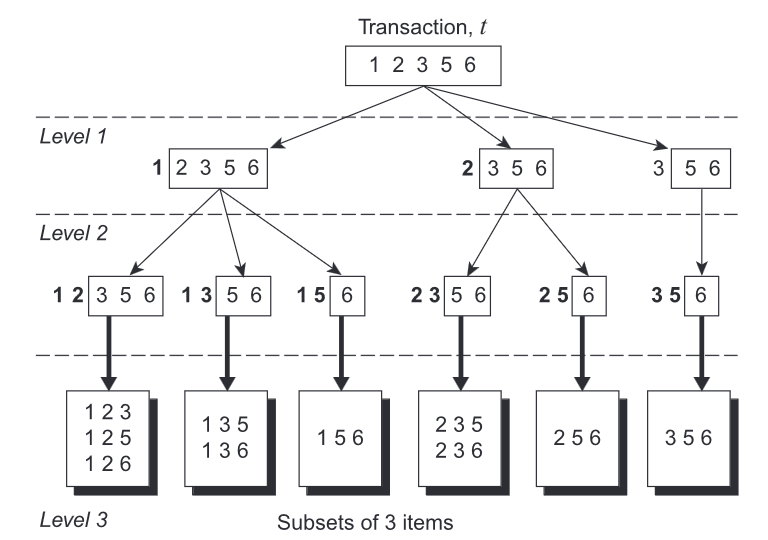
\includegraphics[width=0.7\linewidth]{img/apriori_prefixtree.png}   
\end{figure}

\section{Rule Generation}

Each frequent $k$-itemset, $Y$, can produce up to $2^k - 2$ association rules, excluding rules with empty antecedents or consequents. An association rule can be extracted by partitioning the itemset $Y$ into two non empty subsets, $X$ and $Y-X$, such that $c(X \rightarrow Y_X)$ is greater than \textit{minconf}. Computing the confidence of an association rule does not require additional scans of the transaction dataset. The itemsets from which rules are extracted from are all frequent, and so are their subsets.

Below is the pseudocode of the algorithm.

\begin{algorithm}
\caption{Rule generation of the Apriori algorithm.}
\begin{algorithmic}[1]
    \State TODO
\end{algorithmic}
\end{algorithm}

TODO